%%use beamer to create a presentation
%%high energy physics class final project
%%topic : YM instantons
\documentclass[10pt]{beamer}
\usepackage{graphicx}
\usepackage{amsmath}
\usepackage{amssymb}
\usepackage{slashed}
\usepackage{hyperref}
\usepackage{tikz}
\usepackage{pgfplots}
\usepackage{subcaption}
\usepackage{tikz-feynman}
\usepackage{tikz-3dplot}
\usepackage{tikz-cd}
\usepackage{physics}
\usepackage{cancel}
\usepackage{color}
\usepackage{listings}
\usepackage[export]{adjustbox}
\usepackage{amsfonts}
\usepackage{graphicx} % Required for inserting images
\usepackage{amsthm}
\usepackage[scr=rsfs]{mathalpha}

\newtheorem{defn}{Definition}
\newtheorem{thm}{Theorem}
\newtheorem{lem}{Lemma}
\newtheorem{prop}{Proposition}
\newtheorem{rem}{Remark}
\newtheorem{nte}{Note}
\newtheorem*{exa}{Ex)}





\usetheme{metropolis}
\usecolortheme{beaver}

\title{Yang-Mills Instantons}
\author{Seongmin Kim, Taeyoon Kim}
\institute{SNU}
\date{\today}

\begin{document}

\frame{\titlepage}

%%copilot should give 기본 구조 of each page, \begin{frame} \frametitle{} \begin{itemize} \item \end{itemize} \end{frame}
\begin{frame}
\frametitle{Table of Contents}
%% 1. What is instanton?
%% 2. Instanton effect in Path Integral
%% 3. Yang-Mills Instanton : topology, and Anomalies
%% 4. Effects of Instantons in real world
%% 5. Calculation of Instanton effects
%% 6. Conclusion
\begin{itemize}
\item What is an Instanton?
\item Instanton effect in Path Integral
\item Solitons
\item Yang-Mills Instanton
\item Effects of Instantons in real world
\item Numerical results for a Toy Model
\item BPST instanton
\item Instanton Moduli space
\item Conclusion
\end{itemize}
\end{frame}

\begin{frame}
\frametitle{What is instanton?}
\begin{itemize}
\item Mathematicaly, Instanton is a solution to the classical field equations of motion in Euclidean space.
\begin{equation}
    \delta S_E [\psi_{\text{inst}}] = 0 \rightarrow \text{Euler-Lagrange equation}
\end{equation}
\item Instanton solutions of Euclidean EL equation are localized in (Euclidean) space and time, and have finite (Euclidean) action.
\item In Minkofski QFT, it gives a non-perturbative effect: the tunneling between the classical vacua.
\item Instantons are important in understanding non-perturbative effects and tunneling between vacua in quantum field theory.
\end{itemize}
\end{frame}

\begin{frame}
\frametitle{Instanton effect in Path Integral}
\begin{itemize}
\item In path integral formalism, instantons are classical solution, i.e., the saddle points of the action.
\item Instantons only show up in the Euclidean path integral.
\item Is it physically meaningful? Do we have to consider this effect in Minkowski space QFT?
\item So the path integral is dominated by the instanton contributions in the semiclassical limit.
\item The full path integral is given by the sum of all instanton contributions, with small fluctuations around them.
\end{itemize}
\begin{equation}
Z = \int \mathcal{D}\phi e^{-S[\phi]} = \sum_{\text{instantons}}  e^{-S_{\text{inst}}} \int \mathcal{D}\delta\phi e^{-S_{\text{fluct}}[\delta\phi]}
\end{equation}
\end{frame}
\begin{frame}
    \frametitle{Instanton effect in Path Integral : Example}
    \begin{itemize}
    \item A simple example: the one-dimensional quantum mechanics with two minima.
    \item The potential is given by $V(x) = \frac{1}{2}x^4 - \frac{1}{2}x^2$, and the action is $S = \int dt \left(\frac{1}{2}\dot{x}^2 - V(x)\right)$.
    \item The Euclidean action is $S_E = \int d\tau \left(\frac{1}{2}\dot{x}^2 + V(x)\right)$, and the Euclidean EOM has a classical solution, starting from $x = -1$ at $\tau = -\infty$ and ending at $x = 1$ at $\tau = \infty$.
    \item To evaluate correct path integral, We need to consider all the posible semiclassical paths, including the instanton solution. for example,
    \item If  $T \gg t_{\text{inst}}, $all the instanton solution can be approximated as a composition of $n$ single instanton solution, at time $t_1, ... t_n$, and the instanton action is given by $S = \sum_{i=1}^n S_{\text{inst}}=nS_{\text{inst}}$.

    \end{itemize}
    %% the matrix element of e^(-HT) from x = -1 to x = 1, using the path integral including instanton solution.
    %% small font size
    
\end{frame}
\begin{frame}
    \frametitle{Instanton effect in Path Integral : Calculation}

    So, now we can calculate the matrix element of $e^{-HT}$ from $x = -1$ to $x = 1$, using the path integral including instanton solution.
    \begin{align*}
    \small
    \langle 1 | e^{-HT} | 1 \rangle = \int \mathcal{D}x e^{-S_E} = \sum_{\text{instantons}} e^{-S_{\text{inst}}} \int \mathcal{D}\delta x e^{-S_{\text{fluct}}} \\
    = e^{-T/2} \sum_{n \text{ odd}} \int_{-T/2}^{T/2} d\tau_1 \int_{-T/2}^{\tau_1} d\tau_2 \cdots \int_{-T/2}^{\tau_{n-1}} d\tau_n e^{-nS_{\text{inst}}} \int \mathcal{D}\delta x e^{-S_{\text{fluct}}} 
    \end{align*}


Here, the fluctuation path integral can be factorized into $n$ parts, which are the fluctuation path integrals around each instanton solution.
\begin{align*}
\small
\int \mathcal{D}\delta x e^{-S_{\text{fluct}}} &= \left(\int \mathcal{D}\delta x_n e^{-S_{\text{fluct}}}\right)^n e^{-T/2}= K^n e^{-T/2} \\
    \langle 1 | e^{-HT} | 1 \rangle &= e^{-T/2} \sum_{n \text{ odd}} \int_{-T/2}^{T/2} d\tau_1 \int_{-T/2}^{\tau_1} d\tau_2 \cdots \int_{-T/2}^{\tau_{n-1}} d\tau_n (Ke^{-S_{\text{inst}}})^n \\
    \langle 1 | e^{-HT} | 1 \rangle &=e^{-T/2} \sum_{n \text{ odd}} \frac{1}{n!} K^n(e^{-S_{\text{inst}}})^n T^n = e^{-T/2} \sinh(KTe^{-S_{\text{inst}}}) \\
\end{align*}
\end{frame}

\begin{frame}
\frametitle{Instanton effect in Path Integral : Conclusion}
\begin{itemize}
\item The Path integral including instanton solution gives the correct matrix element of $e^{-HT}$ from $x = -1$ to $x = 1$: $\langle 1 | e^{-HT} | -1 \rangle = e^{-T/2} \sinh(KTe^{-S_{\text{inst}}})$.
\item By changing the result to $T \rightarrow it$, we can get the propagator of the Minkowski QM: $\langle 1 | e^{-iHT} | -1 \rangle = e^{-it/2} \sin(Kte^{-S_{\text{inst}}})$.
\item No instanton solution in Minkowski space, but the instanton effect is still important in understanding the non-perturbative effects in Minkowski QFT.
\item Amplitube $\langle 1 | e^{-iHT} | -1 \rangle = e^{-it/2} \sin(Kte^{-S_{\text{inst}}/\hbar})$ is non-perturbative in $\hbar$, and the instanton effect is essential in understanding the non-perturbative effects in quantum field theory.
\end{itemize}
\end{frame}




\begin{frame}
\frametitle{Solitons}
\begin{itemize}
\item Solitons are the localized, finite energy solutions of the classical field equations of motion.
\item Solitons ARE NOT instantons, but they are related to instantons.
\item Instantons are localized in Euclidean space and time, and have finite Euclidean action.
\item Solitons are localized in space, but stationary in time, and have finite energy.

\end{itemize}

%%%%%%%%%%% 사진 넣ㄴ어야함
\end{frame}
%new page
\begin{frame}
\frametitle{Yang-Mills Instanton : Introduction}
\begin{itemize}
\item Yang-Mills instantons are the instanton solutions of the Yang-Mills theory.
\item The Yang-Mills action is given by $S = \int d^4x \left(-\frac{1}{4g^2}F_{\mu\nu}^a F^{\mu\nu a}\right)$, and the Euclidean action is $S_E = \int d^4x \left(\frac{1}{4g^2}F_{\mu\nu}^a F^{\mu\nu a}\right)$.
\item The Euclidean EOM is given by $\mathcal{D}_\mu F^{\mu\nu a} = 0$, with the Bianchi identity $\sum_{\text{cyc}}\mathcal{D}_\mu \tilde{F}^{\nu\rho a} = 0$.
\item The YM instanton solution is nontrivial solution of the EOM, and can be obtained by solving the self-dual equation $\tilde{F}^{\mu\nu a} = F^{\mu\nu a}$.
%% 공변미분 D 글씨체 \mathcal{D}
\end{itemize}
\end{frame}

\begin{frame}
    \frametitle{Yang-Mills Instanton : Self-dual equation}
    \begin{itemize}
    \item Hodge dual operator : $\tilde{F}^{\mu\nu a} = \frac{1}{2}\epsilon^{\mu\nu\rho\sigma}F_{\rho\sigma}^a$.
    \item The self-dual equation is given by $\tilde{F}^{\mu\nu a} = F^{\mu\nu a}$.
    \item All the 2-forms can be decomposed into self-dual and anti-self-dual parts: $F^{\mu\nu a} = F^{\mu\nu a}_+ + F^{\mu\nu a}_-$.
    \item If either $F^{\mu\nu a}_+$ or $F^{\mu\nu a}_-$ is zero, the solution is called self-dual or anti-self-dual, and satisfies the EOM of the YM theory, $\mathcal{D}_\mu F^{\mu\nu a} = 0$.
    %% 공변미분 D 글씨체 \mathcal{D}
    \end{itemize}
    \end{frame}

\begin{frame}
        \frametitle{Yang-Mills Instanton : evaluating $S_{\text{inst}}$}
        \begin{itemize}
        \item The instanton action is given by $S_{\text{inst}} = \int d^4x \left(\frac{1}{4g^2}F_{\mu\nu}^a F^{\mu\nu a}\right)$.
        \item The action can be evaluated easily when the instanton is self-dual or anti-self-dual.
        \end{itemize}
        \begin{align*}
        S_{\text{YM}} &= \int d^4x \left(\frac{1}{4g^2}F_{\mu\nu}^a F^{\mu\nu a}\right) \\
        &=  \frac{1}{4g^2} \int d^4x \left(F_{\mu\nu}^a \pm \tilde{F}_{\mu\nu}^a\right)^2 \mp \frac{1}{2g^2} \int d^4x \tilde{F}_{\mu\nu}^a F^{\mu\nu a} \\ 
        &\geq \pm \frac{1}{2g^2} \int d^4x \tilde{F}_{\mu\nu}^a F^{\mu\nu a} = \frac{8\pi^2}{g^2}|n|
        \end{align*}
        So, the instanton action is the bound, $8\pi^2|n|/g^2$, where $n$ is the instanton number(the 2nd chern number).
        
        \end{frame}

\begin{frame}
\frametitle{Yang-Mills Instanton : Physical effects}
\begin{itemize}
\item The instanton solution is a non-perturbative effect in the YM theory : $e^{-S_{\text{inst}}}=e^{-8\pi^2|n|/g^2}$ is the tunneling amplitude between the classical vacua, and non-perturbative in $g$.
\item The instanton is a source of tunneling between classical vacua in the YM theory, and the true vaccume structure of the YM theory.
\item THe instanton solution is also important in understanding the $\theta$ term and strong CP problem in the QCD.
\end{itemize}
\end{frame}
\begin{frame}
    \frametitle{Tunneling Effects in YM and QCD : $\theta$-vacuum}
    \begin{itemize}
    \item Classical vaccume of the YM theory?
    \item The YM Hamiltonian is : 
    \item So, there is only one classical vaccume, $F_\mu = 0$, and the vaccume energy is zero.
    \item Then, what tunneling effect appears in the YM theory?
    \end{itemize}
    \end{frame}


\begin{frame}
    \frametitle{Easy example : QM on a circle}
    \begin{itemize}
    \item Consider the quantum mechanics on a circle, with the potential $V(x) = -\cos(x)$.
    \item There is one classical vaccume, $x = 0$, and the vaccume energy is $V(0) = -1$.
    \item But, in path integral formalism, the tunneling effect appears : paths with non-zero winding number.
    \item This contribution can be interpreted as the tunneling to itself, and the tunneling amplitude is given by $e^{-S_{\text{inst}}/\hbar}$.
    \item The tunneling amplitube is non-perturbative in $\hbar$, and this instanton effect gives non-perturbative corrections to the vacccume energy.
    \end{itemize}
    \end{frame}

\begin{frame}
    \frametitle{The theta-term}
    \begin{itemize}
    \item One can consider A "trivial term" aplied to abouve QM on a circle : $S= \int dt \left(\frac{1}{2}\dot{x}^2 + \cos(x) + \frac{\theta}{2\pi} \dot{x}\right)$.
    \item Classicaly, this term is a total derivative, and has no effect on the classical dynamics : the Hamiltonian is the same.
    \item Quantum mechanically : There is no effect in feynmann diagrams, no effect in the perturbative expansion in $\hbar$.
    \item This theta term affects the tunneling probability amplitude between the vaccua, and the non-perturbative correction changes dramatically with the theta term.
    \item the tunneling amplitude gets a phase factor : $e^{-S_{\text{inst}}/\hbar} \rightarrow e^{-S_{\text{inst}}/\hbar + i\theta n}$.
    \end{itemize}
    \end{frame}


\begin{frame}
    \frametitle{The theta-term : Continued}
    \begin{itemize}
    \item The path integral calculation, including the theta term, can be done same as before, using the dilute gas approximation.
    \item The correction term to the vaccume energy is given by $\Delta E \propto -\text{cos}(\theta)e^{-S_{\text{inst}}/\hbar}$.
    \item In the wavefuncion picture, this theta term affects the ground state energy by changing the boundary condition of the wavefunction : $\psi(x+2\pi) = e^{i\theta}\psi(x)$.
    \item We numerically calculated the vaccume energy of the QM on a circle, and the result is consistent with the path integral calculation.
    \end{itemize}
    \end{frame}


\begin{frame}
    \frametitle{The theta-term : Numerical Calculation}
    %% put fig : E_G, E_G_diff
    %% 두 그림을 서로 옆에 두기
        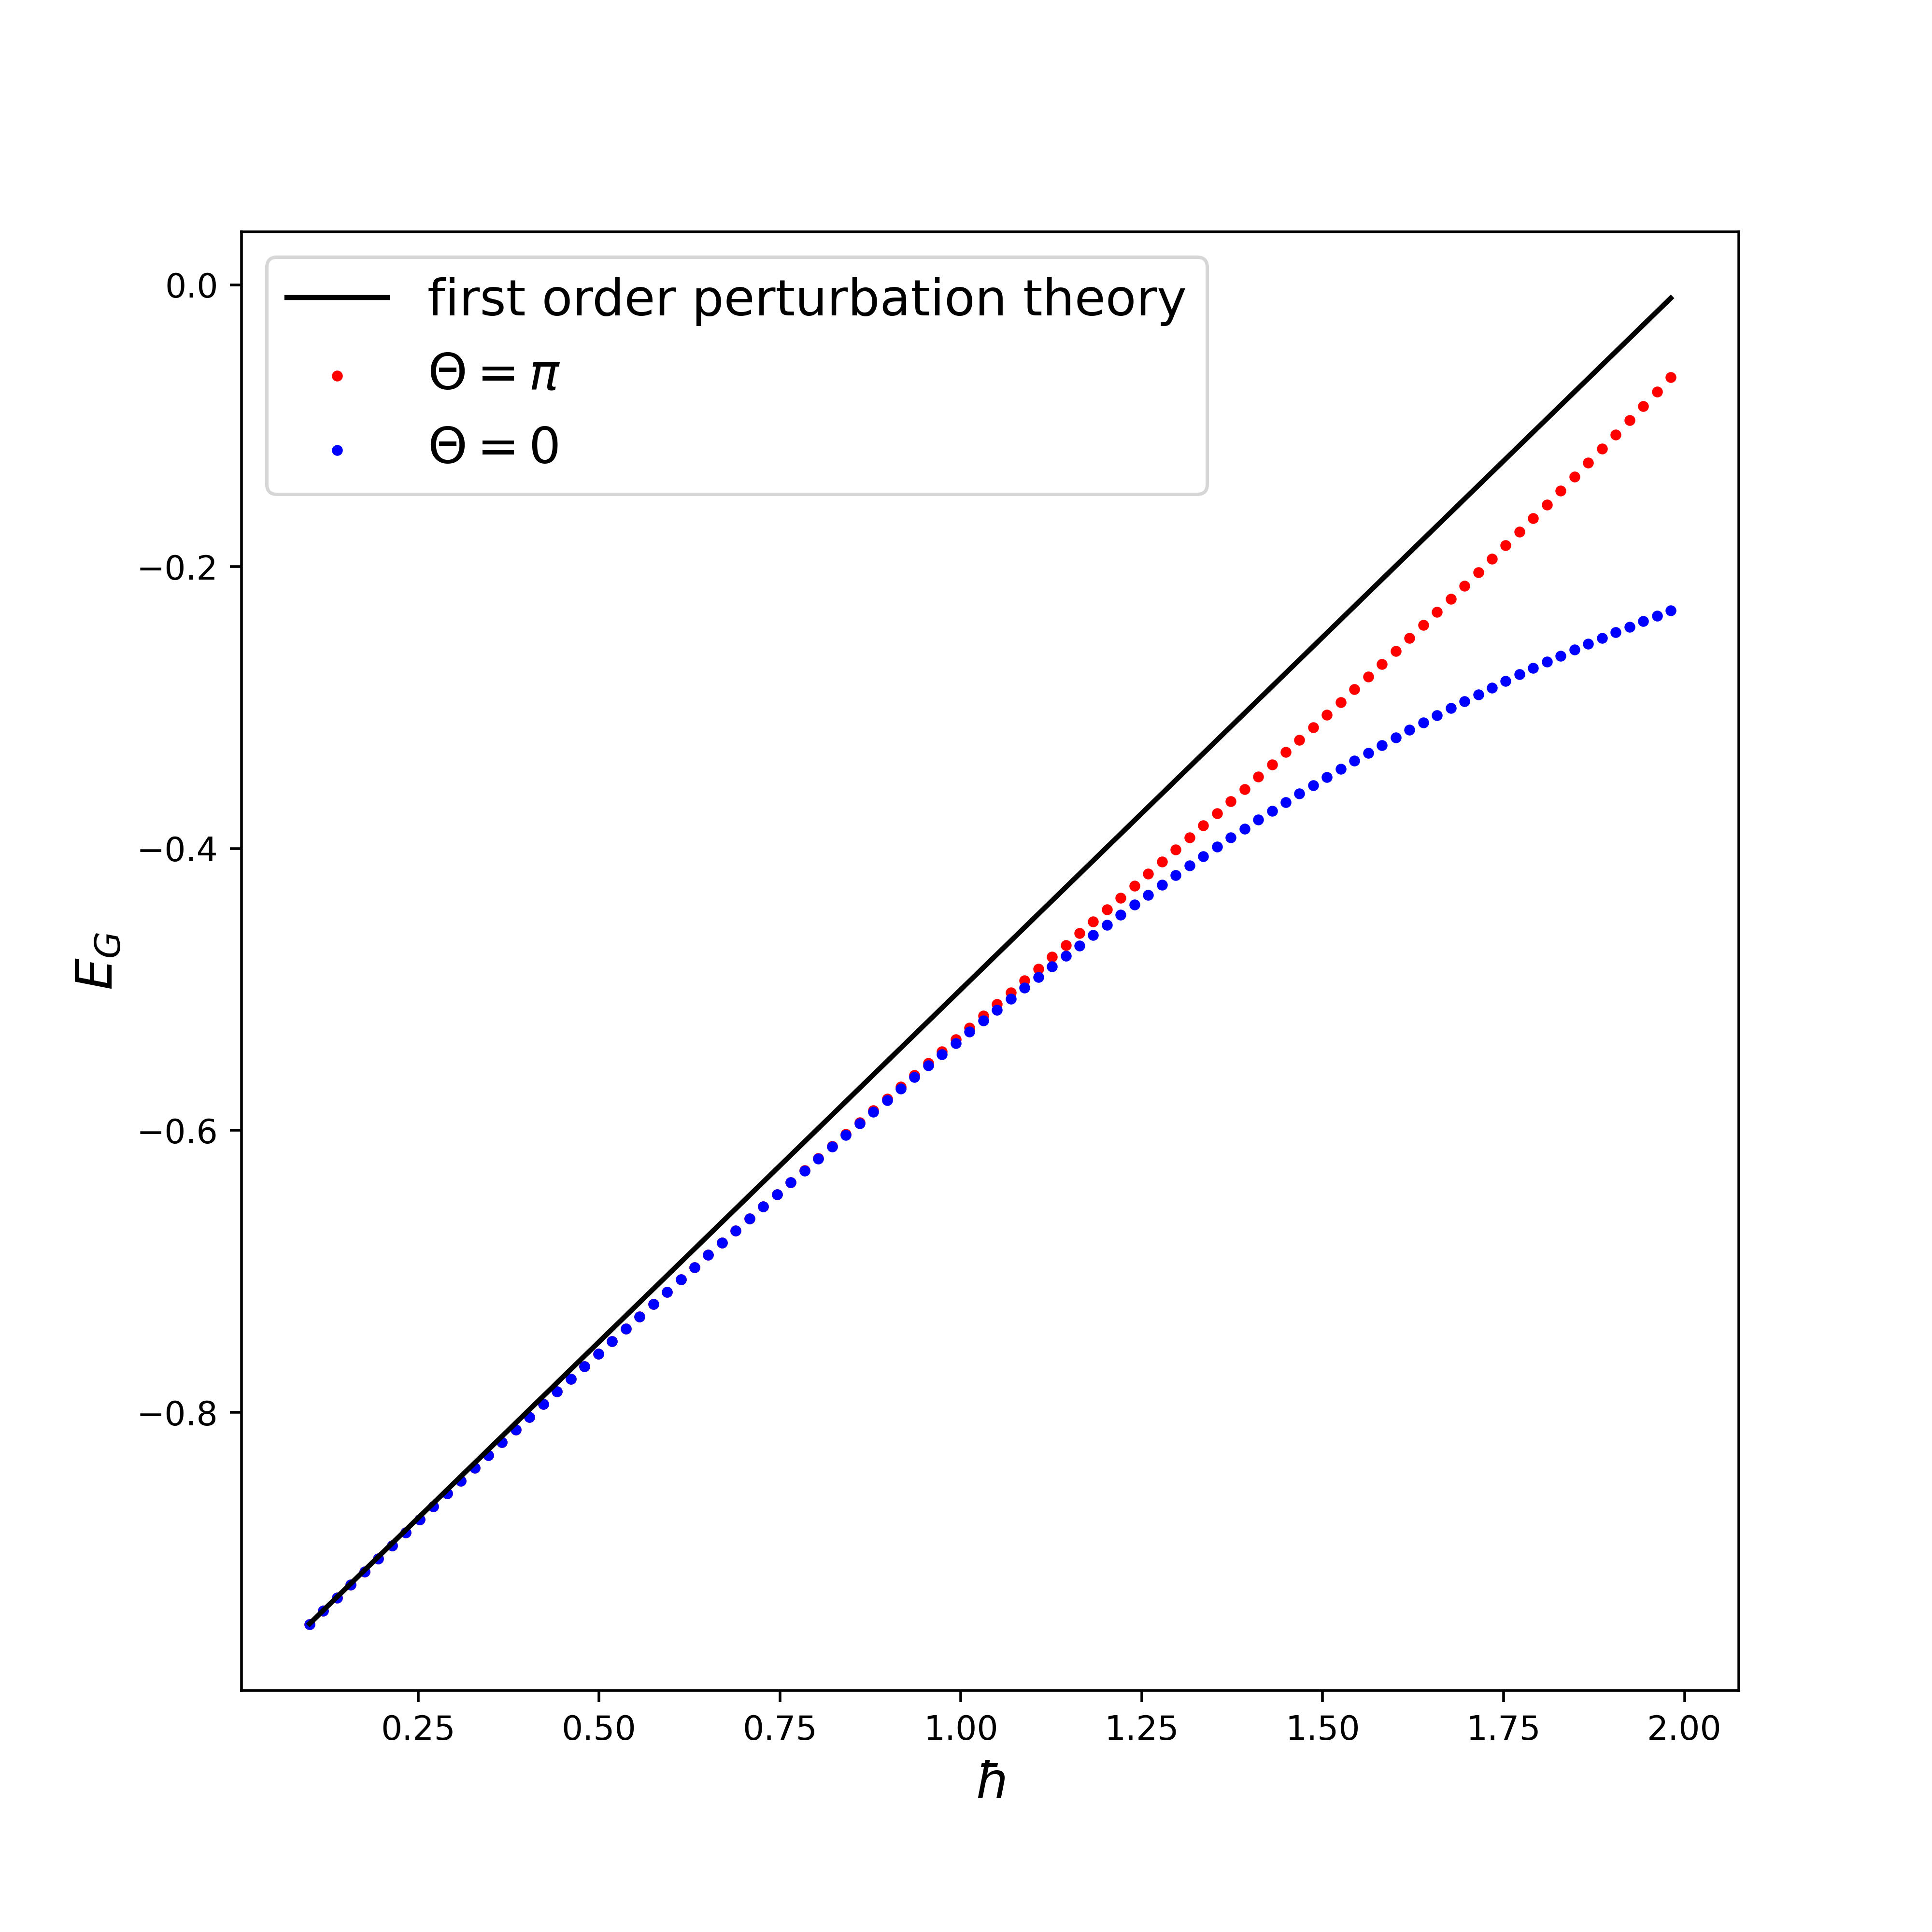
\includegraphics[width=0.6 \textwidth]{E_G.png}

        $\Delta E \propto -\text{cos}(\theta)e^{-S_{\text{inst}}/\hbar}$
\end{frame}

\begin{frame}
    \frametitle{The theta-term : Numerical Calculation}

       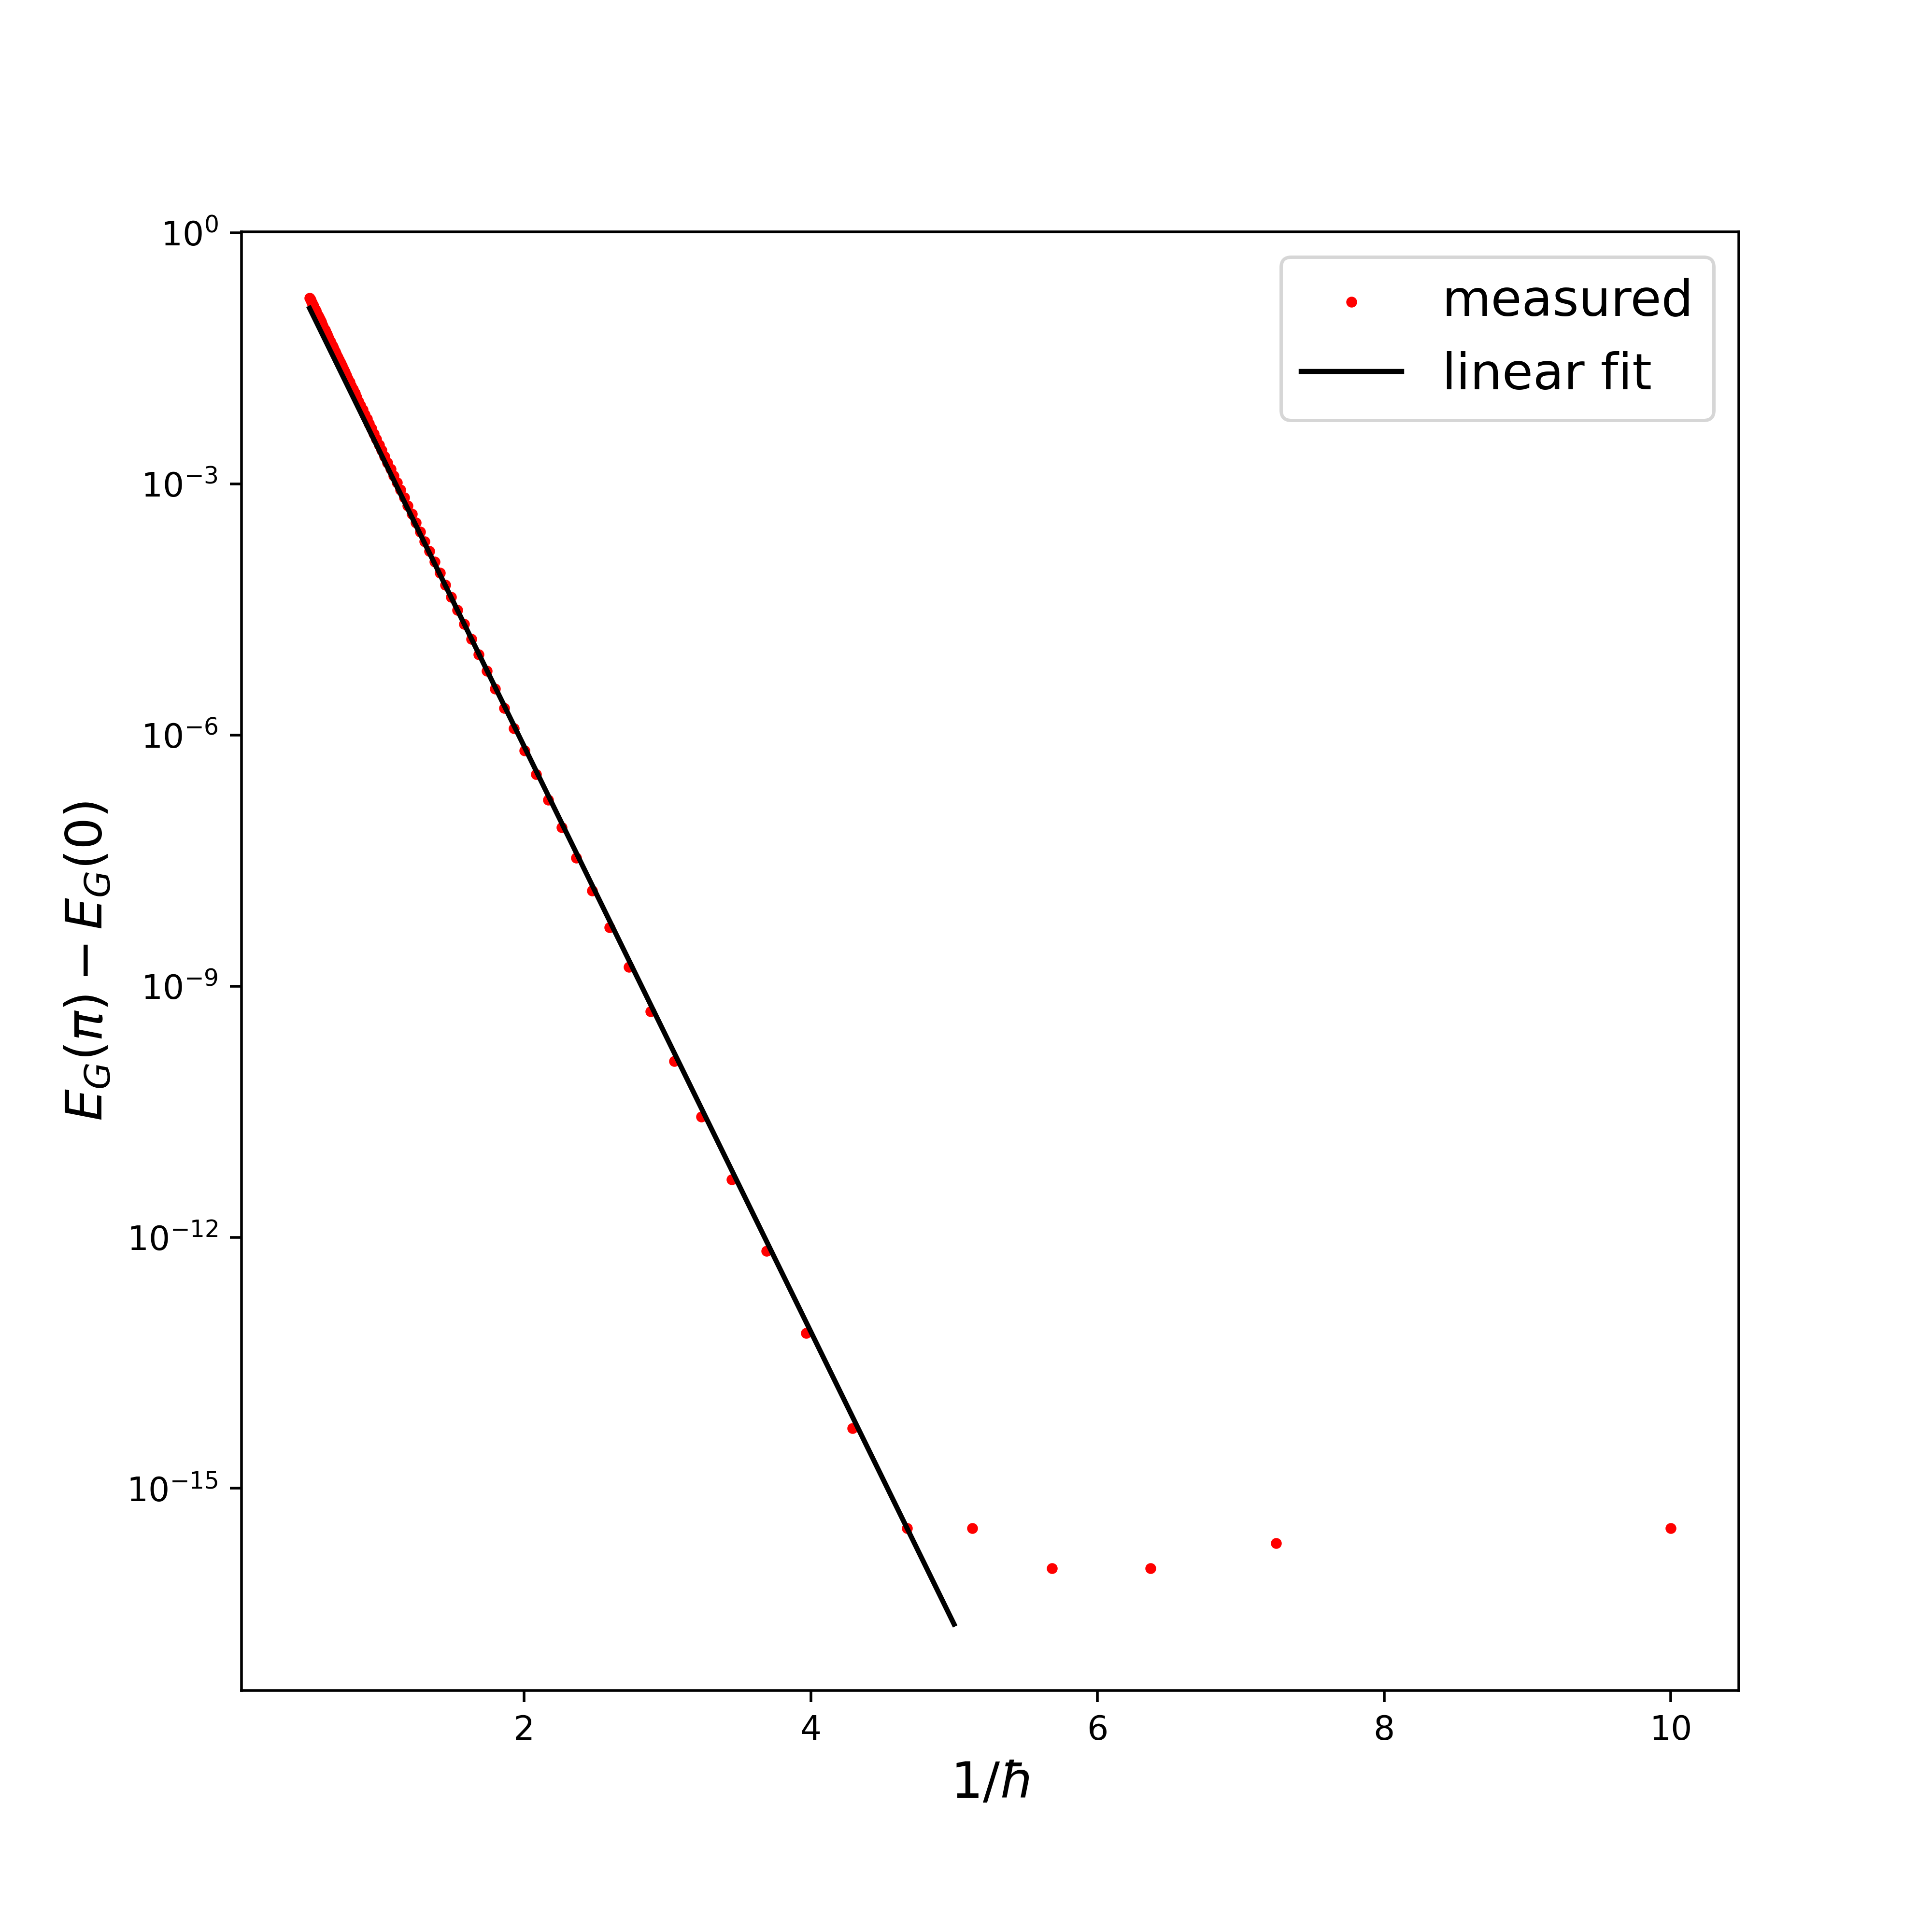
\includegraphics[width=0.6\textwidth]{E_G_diff.png}

     $\Delta E \propto -\text{cos}(\theta)e^{-S_{\text{inst}}/\hbar}$, \ \ \ 
     $S_{\text{inst}} = \int_0^{2\pi} dx \left(2-2\text{cos}(\theta)\right)^{1/2}=8$
    \end{frame}

\begin{frame}
    \frametitle{The theta-term : Conclusion}
    \begin{itemize}
    \item The instanton effect and the theta term in the QM on a circle changes the vaccume energy, and the vaccume structure of the theory.
    \item The energy correction is non-perturbative in $\hbar$, asympotically : $\Delta E \propto -e^{-S_{\text{inst}}/\hbar}\text{cos}(\theta)$.
    \item The theta term changes the vaccume energy by changing the phase of the instanton Amplitude
    \item In wavefunction picture, the theta term changes the boundary condition of the wavefunction.
    \end{itemize}
\end{frame}

\begin{frame}
    \frametitle{The QCD theta term}
    \begin{itemize}
    \item The theta term in QCD is given by $S_{\theta} = \frac{\theta}{32\pi^2}\int d^4x \epsilon^{\mu\nu\rho\sigma}F_{\mu\nu}^a F_{\rho\sigma}^a$.
    \item The theta term is a total derivative, and has no effect on the classical dynamics, or perturbative QM of the QCD.
    \item But, the theta term affects the non-perturbative effects of the QCD, and the vaccume structure of the QCD.
    \item The theta term affects the vaccume energy of the QED, by changing the phase of the YM instanton amplitude.
    \end{itemize}
    \begin{equation}
        e^{-\frac{8\pi^2}{g^2}|n|} \rightarrow e^{-\frac{8\pi^2}{g^2}|n| + i\theta n}
    \end{equation}
\end{frame}

\begin{frame}
    \frametitle{Effects on Real world physics}
    \begin{itemize}
    \item The theta term only affects the non-perturbative effects of the QCD.
    \item At high energy scales, the theta term is not important, since the QCD is asymptotically free.
    \item At low energy scales, QCD is confining, and the theta term is important. All the things are non-perturbative!
    \item The theta term changes the vaccume energy of the QCD, the electric dipole moment of the neutron, ....
    \end{itemize}
\end{frame}

\begin{frame}{BPST solution}
    For self dual instanton on $\mathbb{R}^4$, Use the ansatz while $\sigma_{\mu\nu}$ are generators for rotation in Euclidean $\mathbb{R}^4$, Projected to the left handed part. 
    
    Then $\sigma_{\mu\nu}$ are $SU(2)$ generators, satisfying
    \[
    [\sigma_{\mu\nu},\sigma_{\rho\sigma}] = -2\left(\delta_{\mu \rho} \sigma_{\nu \sigma}+\delta_{\nu \sigma} \sigma_{\mu \rho}-\delta_{\mu \sigma} \sigma_{\nu \rho}-\delta_{\nu \rho} \sigma_{\mu \sigma}\right)
    \]
    \[
        A_{\mu}(x) = \alpha \sigma_{\mu \nu} \partial_{\nu} \mathrm{log} \phi(x^2).
    \]
    \[
        F_{\mu\nu}-\star F_{\mu\nu} = \sigma_{\mu\nu}(-2\alpha^2(\partial\mathrm{log}\phi)^2-\alpha\partial^2\mathrm{log}\phi)
    \]

To equip self duality, $-2\alpha^2(\partial \mathrm{log}\phi)^2 = \alpha\partial^2\phi$ needs to be satisfied. Substituting $\phi\rightarrow\phi^{1/2\alpha}$, one can get that $\phi^{-1}\partial^2\phi=0$, which is just laplace equation.
\end{frame}

\begin{frame}{BPST solution}
    $\phi = \frac{\rho^2}{(x-a)^2}+C$, while $C=1$ so that it goes 0 at infinity.

    \[
    A_\mu(x) = -\sigma_{\mu\nu}\frac{\rho^2(x-a)_\nu}{(x-a)^2((x-a)^2+\rho^2)}
    \]
    With a proper gauge transformation, $U=\frac{i\bar{\sigma}_\mu x_\mu}{|x|}$,
    \[
    U(\partial_\mu +A_\mu )U^{-1} =  -\bar{\sigma}_{\mu\nu}\frac{(x-a)_\nu}{((x-a)^2+\rho^2)}
    \]
    And the induced curvature is as the following.
    \[
         F_{\mu\nu}=\frac{2 \rho^2 \bar{\sigma}_{\mu \nu}}{\left[(x-a)^2+\rho^2\right]^2}
    \]

    Such $\rho$ and $a$ represents the conformal transformation of $\mathbb{R}^4$. Since Hodge star is conformally invariant, they also make solutions.
\end{frame}



\begin{frame}{Instanton Moduli}
    \begin{rem}
        In Classic Yang Mills, $F_\nabla$ must satisfy the following equations. \\
        $d_\nabla^\star F_\nabla =0$(equation of motion), $d_\nabla F=0$(Bianchi identity)
    \end{rem}
    Therefore, $\star F=\pm F$ condition would automatically make equation of motion satisfied. 
\end{frame}


\begin{frame}{Instanton Moduli}

    \begin{thm}[Atiyah-Hitchin-Singer]
        Let $M$ be a compact, self-dual Riemannian manifold with positive scalar curvature. Let $P$ be a principal $G$-bundle over $M$, where $G$ is a compact semisimple Lie group. Then the space of moduli of irreducible self-dual connections is either empty or a manifold of dimension 
        \[
            p_1(\mathfrak{g})-\frac{1}{2}\mathrm{dim}G(\chi-\tau)
        \]
        While $\chi$ is the Euler characteristic of $M$ and $\tau$ is the signature of $M$. 
    \end{thm}

    Throughout, the Instanton itself is crucial as a classic solution of the physical action. The perspective that considering such 'space of connections' fulfills lots of geometries/topologies and physics
\end{frame}



\begin{frame}[fragile]{Sketch of the Proof (AHS)}

    Consider the following chain complex. $d_\nabla^- = p_-d_\nabla$
    \[
        \begin{tikzcd}
        0 \arrow[r] & \Omega^0(M, \mathfrak{g}) \arrow[r, "d_\nabla"] & \Omega^1(M, \mathfrak{g}) \arrow[r, "d_\nabla^{-}"] & \Omega^2_{-}(M, \mathfrak{g}) \arrow[r] & 0
        \end{tikzcd}
    \]

    The first claim is that if $\tau \in T_A\mathscr{A}/\mathscr{G}$ then $\tau\in\mathrm{Im}d$. Consider the following gauge transformation. Taking the local chart and for any lie algebra $X\in\mathfrak{g}$, 
    \[
        A(t) = e^{-tX}A e^{tX} + e^{-tX}d e^{tX}
    \]
    And the differential of the map, i.e. the tangent connection at $A$, is as the following.
    \[
        \left.\frac{d}{dt}\right|_{t=0}A(t)= [X,A] - dX = -d_\nabla X
    \]
    This proves that the element of $T_A\mathscr{A}/\mathscr{G}$ lies in $\mathrm{Im}d_\nabla$. While the self dual connection lies trivially on the kernel of 2nd map
 
\end{frame}

\begin{frame}{Sketch of the Proof (AHS)}
    Therefore the tangent space $T_A\mathscr{A}_+/\mathscr{G}\cong H^1(M,\mathfrak{g})$. The index of the complex is the following. $h_i$s represent the dimensions of cohomologies.
    \[
        \mathrm{ind}D = h_0-h_1+h_2
    \]
    The index of the complex is the index of the following elliptic operator.
    \[
        D=d_\nabla^\star + d_\nabla^-: \Omega^1(M,\mathfrak{g})\rightarrow \Omega^0(M,\mathfrak{g}) \oplus \Omega^2(M,\mathfrak{g})
    \]

    We claim that $h_0=h_2=0$
\end{frame}

\begin{frame}{Instanton Moduli}
    \begin{defn}[Irreducible Connection]
        For a principal $G$-bundle $P$ over a connected manifold $M$, a connection is said to be irreducible, if for some point $x\in M$
        \[
            \mathrm{Hol}(x) = G
        \]
        While $\mathrm{Hol}(x)$ denotes the holonomy group around a point $x$.
    \end{defn}

    \begin{prop}[Covariance of Parallel transport]
        For a gauge transformation $\Phi$, parallel transform, acted by $\Phi$(i.e. the connection is changed) can be written as the following.
        \[
            P^{\Phi}_\gamma = \Phi(\gamma(1))P_\gamma \Phi^{-1}(\gamma(0))
        \]
    \end{prop}

    Therefore, if a connection is irreducible, gauge transformation that fixes the connection must lie on the center. While semisimple lie group admits a 0 dimensional center. (modulo scalar)
    \[
        P^{\Phi}_\gamma = P_\gamma = \Phi(\gamma(0))P_\gamma\Phi^{-1}(\gamma(0))
    \]
\end{frame}

\begin{frame}{Sketch of the Proof (AHS)}
    $H^0(M,\mathfrak{g})=\mathrm{ker}d_\nabla$, which is just constant gauge field, $d_\nabla X=0$. Using the description above, it fixes $A(t)$ and hence 0 dimensional by irreducibility. This proves $h_0=0$.\\
\end{frame}

\begin{frame}[fragile]{Sketch of the Proof (AHS)}
    \begin{nte}[Witzenböck Formula]
        For a covariant exterior derivative $d_\nabla$, 
        \[
            \Delta= d_\nabla^{-} (d_\nabla^{-})^\star = \frac{1}{2}d_\nabla d_\nabla^\star + \frac{R}{6} - W_-
        \]
        $R$ represents the Ricci scalar, and $W_-$ represents the anti self dual part of Weyl tensor.
    \end{nte}
    In our setting, this shows that $d_\nabla^-$ is positive-definite and hence any $\omega\in H^2_-(M,\mathfrak{g})$ is$d_\nabla$ of $d_\nabla^\star\omega$ up to positive constant. Which proves that $h_2=0$.
\end{frame}



\begin{frame}{Sketch of the Proof (AHS)}
    Index can be calculated by Atiyah-Singer Index theorem.
    \[
        \mathrm{ind}D = \int_M \mathrm{ch} \left( \bigoplus_i (-1)^i E_i \right) \frac{\mathrm{Td}(TM \otimes_\mathbb{R} \mathbb{C})}{\mathrm{e}(TM)}
    \]
    The original paper of AHS used equivalence of differential forms and spinor bundle to calculate such index in a simpler way.
    \[
        \mathrm{ind}D = p_1(\mathfrak{g})+\frac{1}{2}\mathrm{dim}G(\chi-\tau)
    \]

    \begin{thm}[$\mathrm{SU}(2)$ bundle over $S^4$]
        For $\mathrm{SU}(2)$ bundle over $S^4$ of $c_2(\nabla)=k$, $\mathrm{ind}D=8k-3$, while $\chi(S^4)=2$, $\tau(S^4)=0$. Hence a moduli space dimension if $8k-3$
    \end{thm}
\end{frame}
\begin{frame}{BPST solution}
  
    The reason why $S^4$ and $\mathbb{R}^4$ make same result is because assumption is $k=1$. Only need to take the hemisphere that doesn't have instanton distribution in it.
     \\
     As a persepective of pure gauge story, the only information about the instanton at infinities are the winding numbers. Which needs to be true, since the action functional $\mathrm{tr}(F\wedge F)$ is locally exact, as $d\mathrm{tr}(A dA + \frac{2}{3}A^3)$. Meaning that for $S^4$ configuration, the stokes theorem gives the information on boundary, as the Chern Simons form.
     \\
     
     
 \end{frame}

\begin{frame}[fragile]{Characteristic Class}
    \[
    \begin{tikzcd}
       \mathrm{Bun}_G(-)/\sim \arrow[r] 
        & {[-,\mathrm{BG}]}\arrow[l] \arrow[d, "Ch.Class"] \\
         & {H^*(-,\mathbb{Z})}
    \end{tikzcd}
    \]
    
    If we are given a data of $\mathrm{Bun}_G(-)/\sim$, there exists a way to have some $H^*(-,\mathbb{R})$. Which is known as the Chern-Weil homomorphism. The only remaining step is to check that such object made by Chern Weil is the characteristic class. The mathematical definition of the Chern class has some axioms, and one can verify if the Chern-Weil satisfies the axioms. This explains an integrality of Chern classes.
     
 \end{frame}
\end{document}